\chapter{Motivation}
\pagenumbering{arabic}

In this chapter we will introduce the very motivation of this work. From medical point of view, this work focuses on a medical condition known as intracranial hemorrhage. We will adduce the elementary facts about this condition for more comprehensive understanding of the whole problematic. Furthermore, an overview of standard approach to the process of diagnostics will be presented.

\section{Intracranial hemorrhage}
Intracranial hemorrhage, commonly referred to as ICH, is a serious and potentially deathly health condition. This type of hemorrhage poses any type of bleeding present within the fixed intracranial vault \cite{intracranial1}. The most common causes of intracranial hemorrhage are a traumatic brain injury as well as spontaneous appearance, due to a vascular malformation, which stands for a disease of the vessel \cite{intracranial2}. If not treated promptly, the hemorrhage can subsequently account for even more serious conditions, such as coma, seizures or stroke. \cite{intracranial2} Strokes can be categorized as hemorrhagic - caused by an intracranial bleeding, and ischemic - result of a blockage in an artery supplying blood to the brain. As stated in the book of Urden er al. \cite{ICHbookstats}, 13\% of all strokes in the United States yearly are hemorrhagic strokes and 87\% are ischemic strokes. Although hemorrhagic strokes occur less frequently, their mortality rate is much higher, with 37\% to 38\% of such cases resulting in death within the first month. After cardiovascular diseases, cancer and chronic respiratory diseases, stroke is the fourth leading death cause in the United States \cite{ICHbookstats}. The number of deaths can be greatly decreased with accurate and precocious diagnosis. 

\subsection{Types of hemorrhage}
Intracranial hemorrhage can be further subdivided into five most common subtypes, varying in the region in which they appear in the intracranium. \cite{ICHsubtypes-CT, imagingICH} These subtypes include intraparenchymal, intraventricular, subarachnoid, subdural and epidural hemorrhage. Figure 2.1 presents examples of CT findings of each of the subtypes respectively. 
% \ref{fig:subtypes}:
\begin{figure}[h]
\begin{centering}
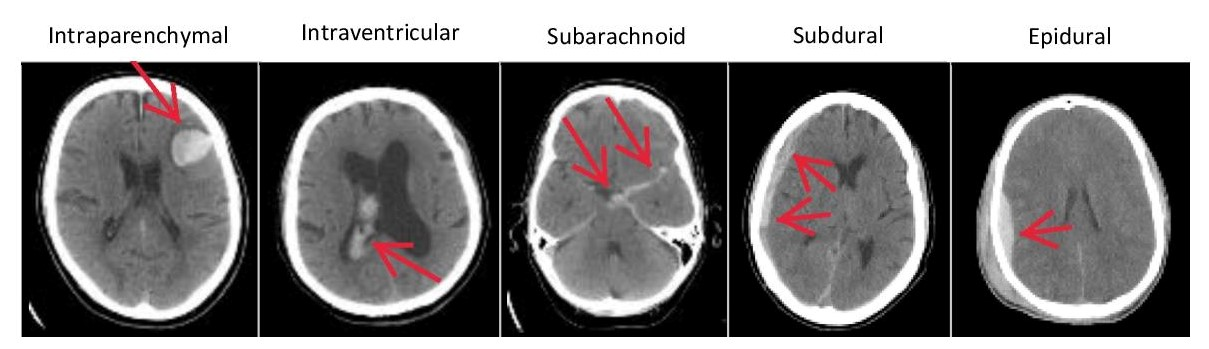
\includegraphics[width=15cm]{assets/images/subtypes}
\par\end{centering}
\caption{Five subtypes of intracranial hemorrhage \label{fig:subtypes}}
\end{figure}

The symptoms of the patient and the severity of the bleeding is dependant on the subtype. \cite{ICHsubtypes-CT}

\section{Diagnostics using computed tompography}
Neuroimaging is crucial when aiming for an exact diagnosis of intracranial hemorrhage. Taking into account its wide availability and non-invasive technique, computed tomography (CT) is conventionally used technique in detection of intracranial hemorrhage these days \cite{imagingICH}. Even though magnetic resonance imaging (MRI) has proven to be more sensitive to detail, CT is able to provide much faster results, which is critical when it comes to obtaining early assessment of the presence as well as extent of the bleeding \cite{imagingAfterBrainInjury}. Computed tomography

